\section{Partial Support for OMNeT++ Links and Protocol
Handshaking}\label{sec:partial-work}

The current \iblock{} implementation lacks support for traditional \omnetpp{}
links, meaning it does not simulate the network's physical layer. Additionally,
it does not fully implement Bitcoin's gossip protocol: instead of propagating
blocks and transactions through the network node-by-node as in a real Bitcoin
network, \iblock{} broadcasts them directly to all nodes.

However, initial steps toward these features have been made. Currently, only
protocol handshaking and a basic ping-pong mechanism are in place, functioning
through \omnetpp{} links.

The following sections detail these preliminary implementations.
\figref{fig:next-uml} on page~\pageref{fig:next-uml} shows the UML diagram of
the relevant classes, while possible future development is outlined in
\chref{ch:next}.

\begin{figure*}
	\centering
	\adjustbox{trim={0} {0} {0.5\width}
	{0},clip}{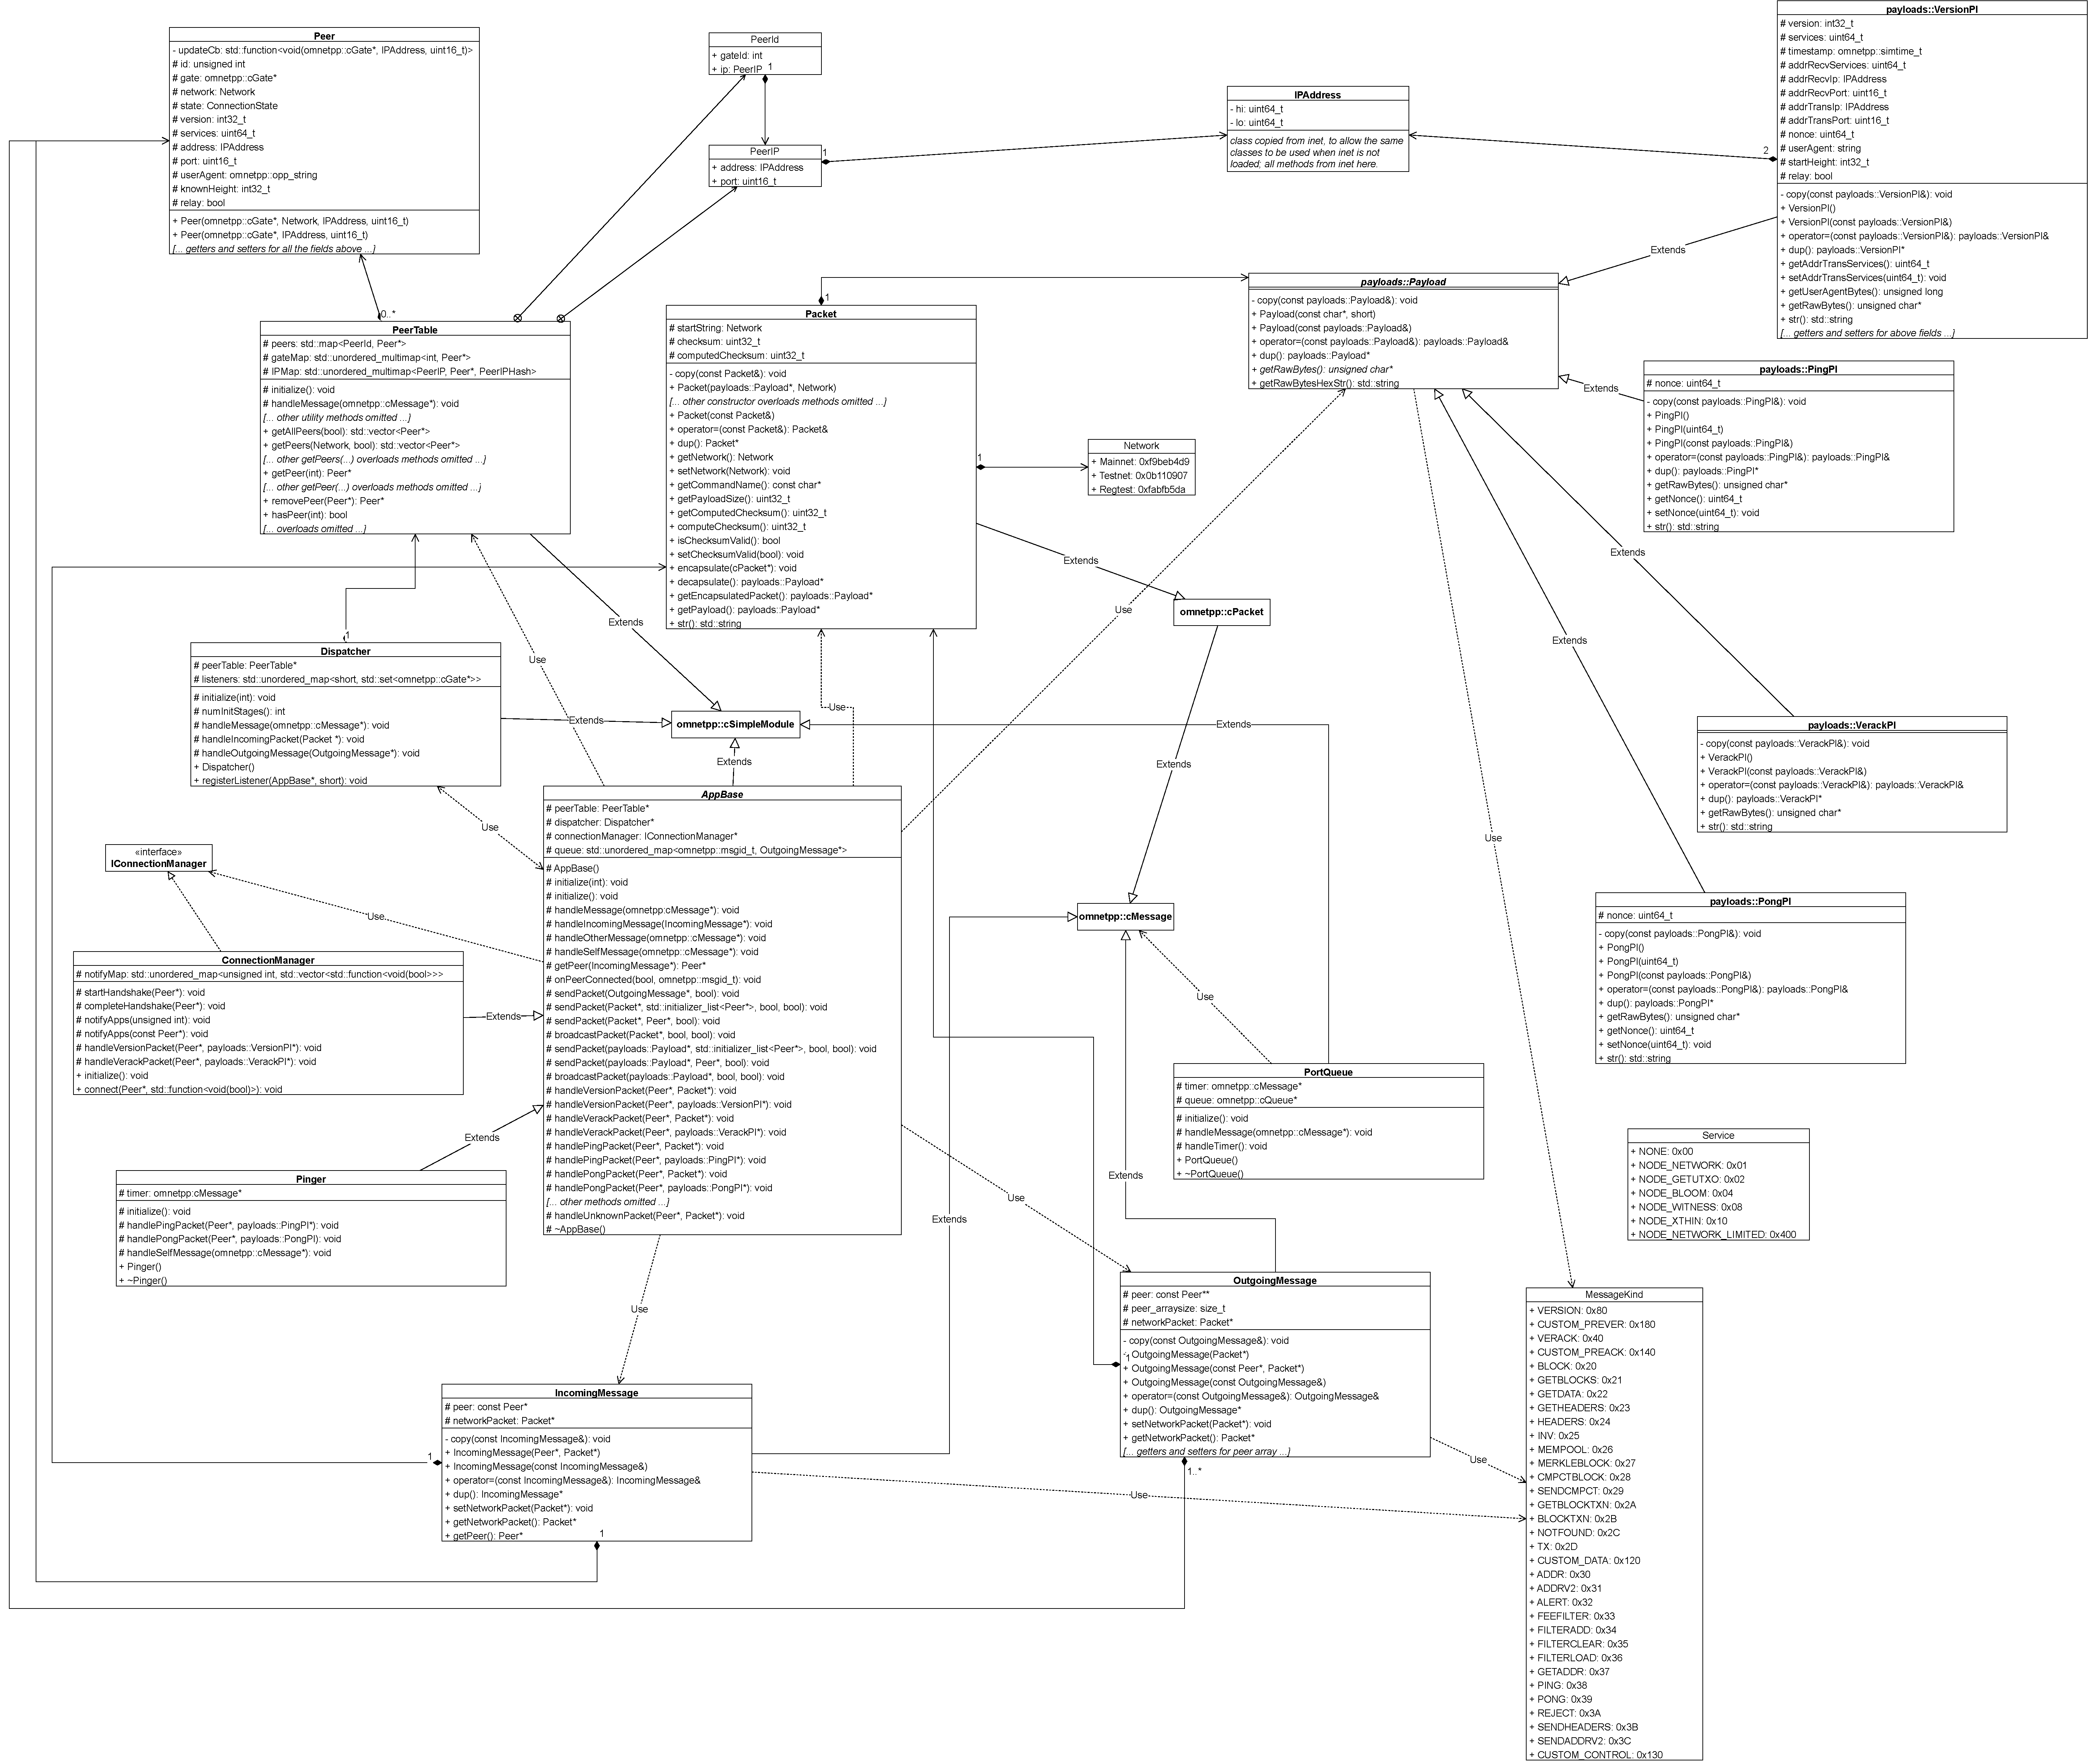
\includegraphics[width=2\textwidth,height=0.9\textheight,keepaspectratio]{next-uml}}
	\phantomcaption
\end{figure*}

\begin{figure*}
	\ContinuedFloat
	\centering
	\adjustbox{trim={0.5\width} {0} {0}
	{0},clip}{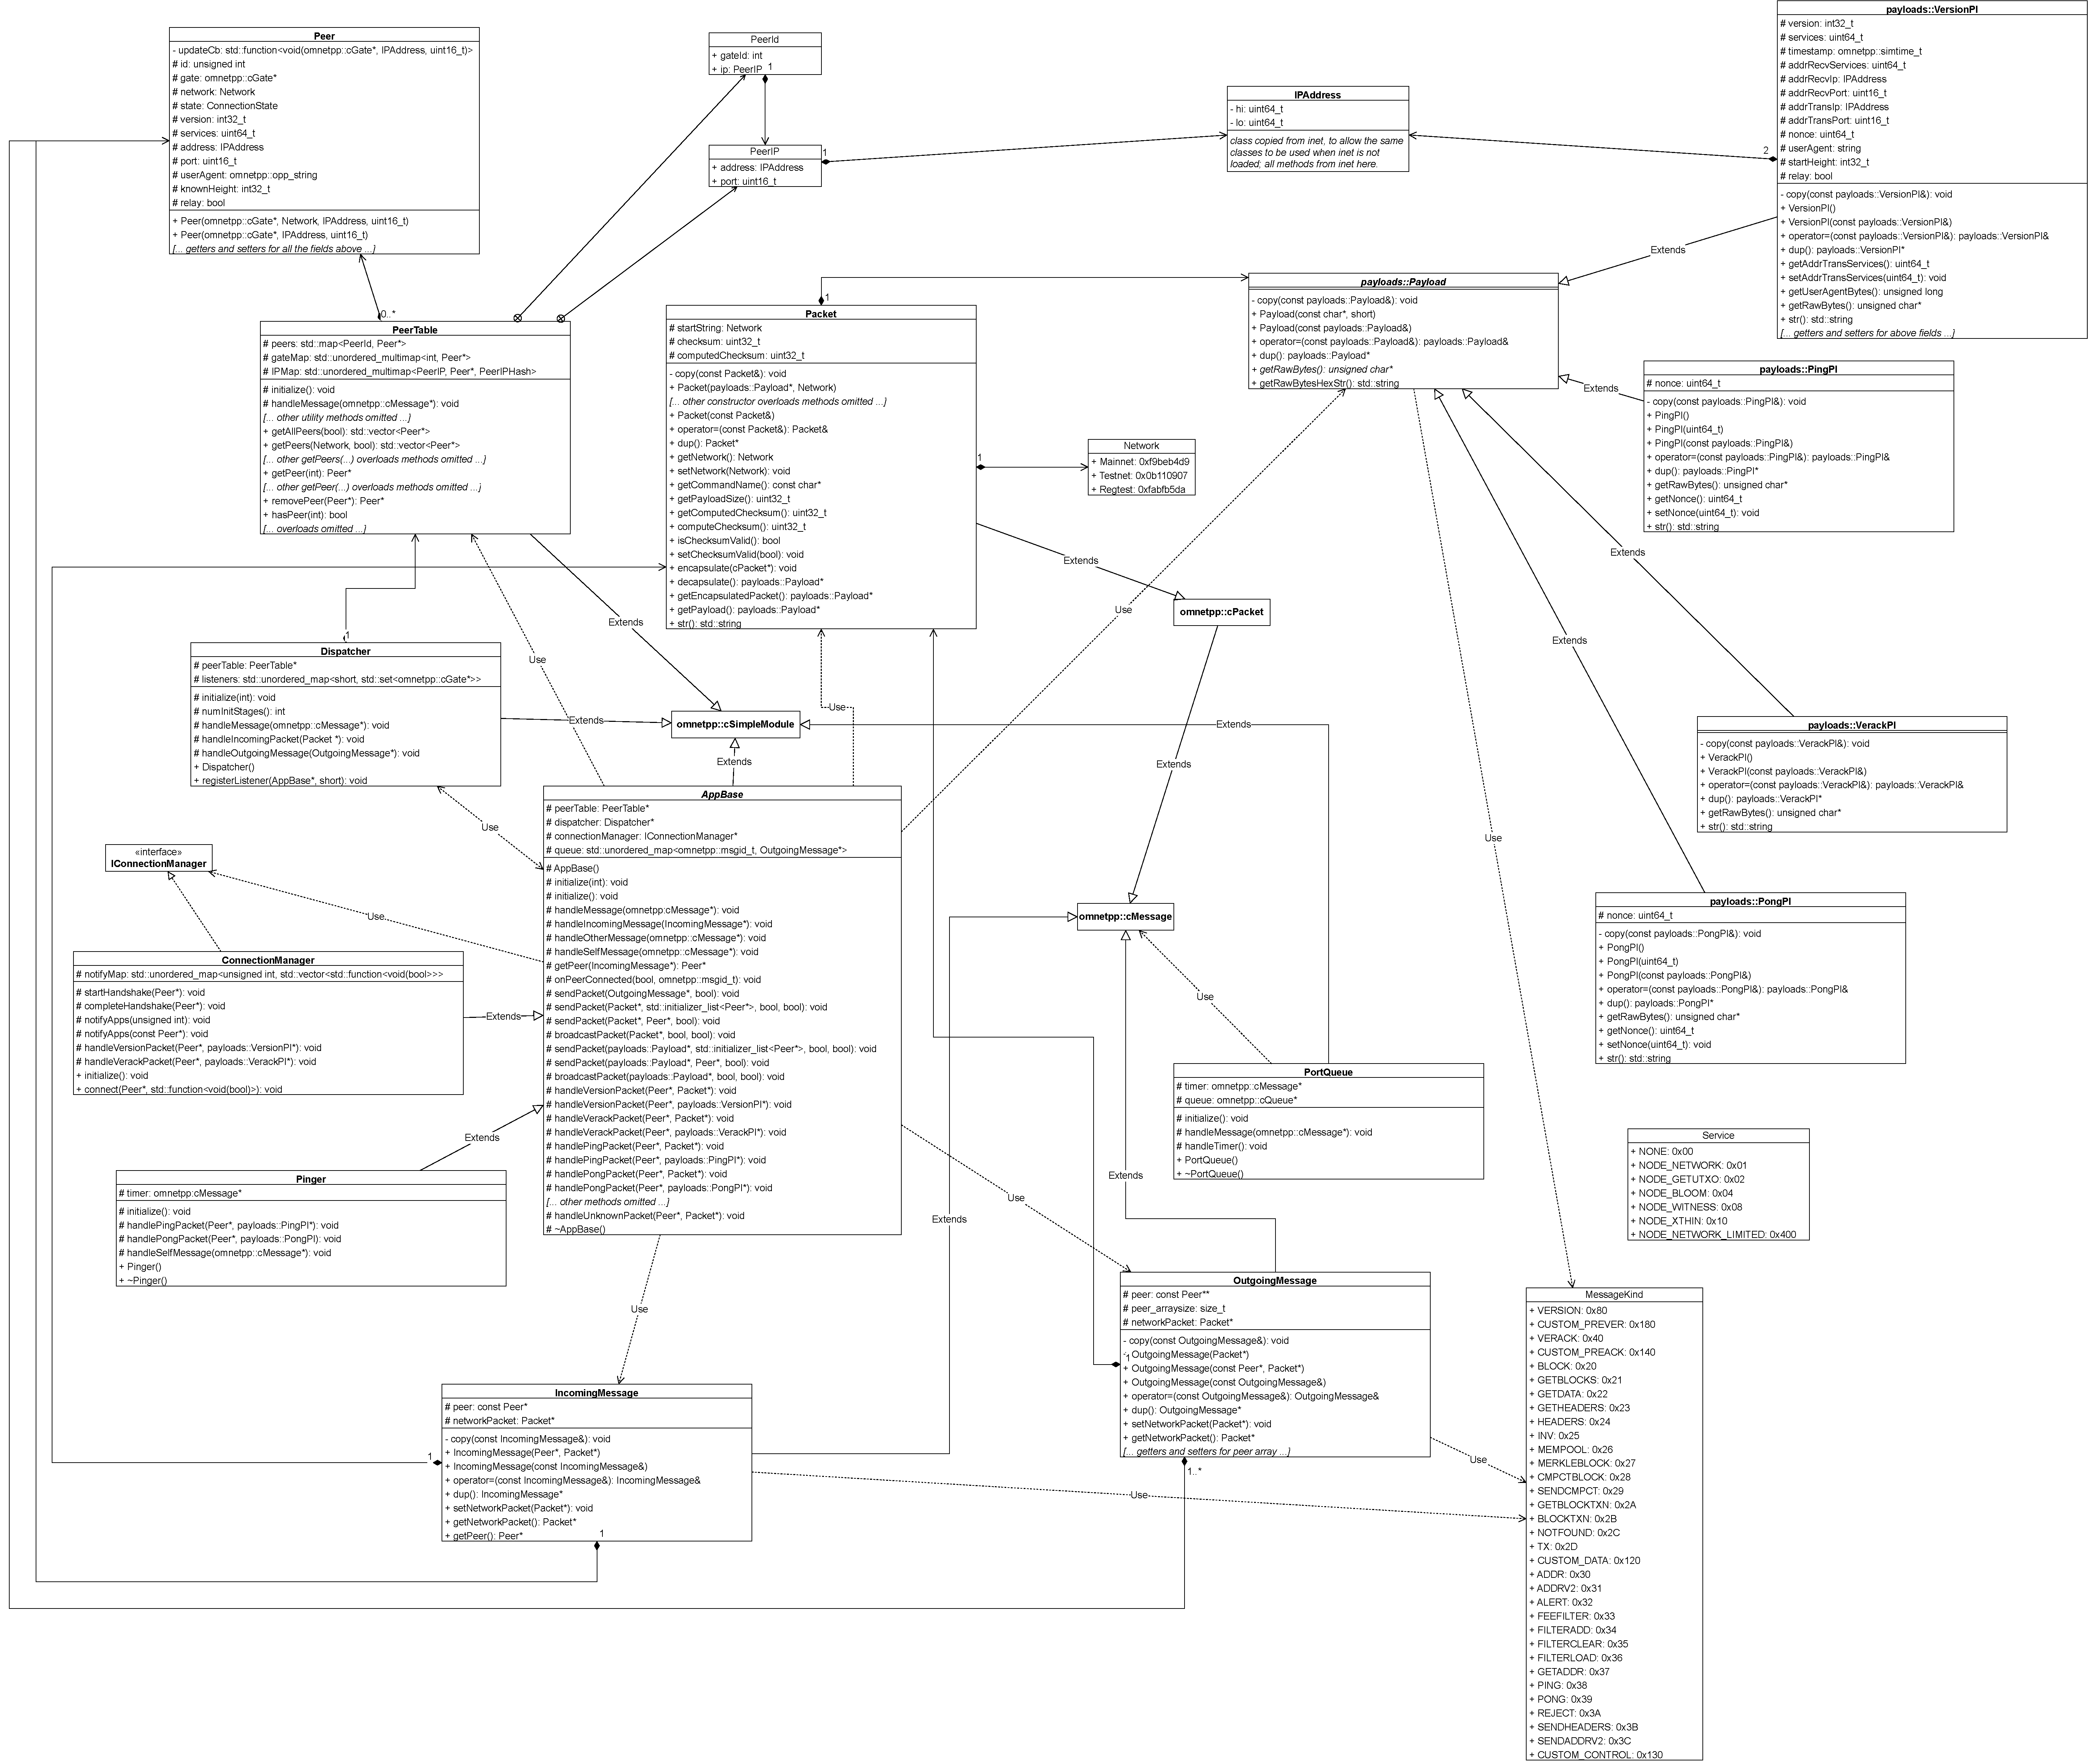
\includegraphics[width=2\textwidth,height=0.9\textheight,keepaspectratio]{next-uml}}
	\caption{UML diagram of the classes discussed in
	\secref{sec:partial-work}.}\label{fig:next-uml}
\end{figure*}

\subsection{Maintaining a List of Peers}\label{subsec:peers-list}

Using \omnetpp{} links means that each node must keep a list of its peers with
informations about them, such as the gate through which they are connected and
the features they support. This list is maintained by the \code{PeerTable}
module, which supports method to add, retrieve, and remove peers.

The peer table will be filled by the \code{ConnectionManager} module, which
handles the initial handshake with other nodes. Each time a node wants to send
a message to one of its peers, the \code{Dispatcher} module will use the
informations in the peer table to determine how to contact the peer.

\subsection{Dispatching Messages to Applications}\label{subsec:dispatcher}

The structure of an \iblock{} node must be altered to allow for messages to be
exchanged using links. \figref{fig:next-node} on page~\pageref{fig:next-node}
shows the new structure of nodes. Blue squares are gates: the user does not
need to manually add them to the node when connecting it to other peers or
adding new applications --- they are added automatically by \omnetpp{}.

\begin{figure}[tbhp]
	\centering
	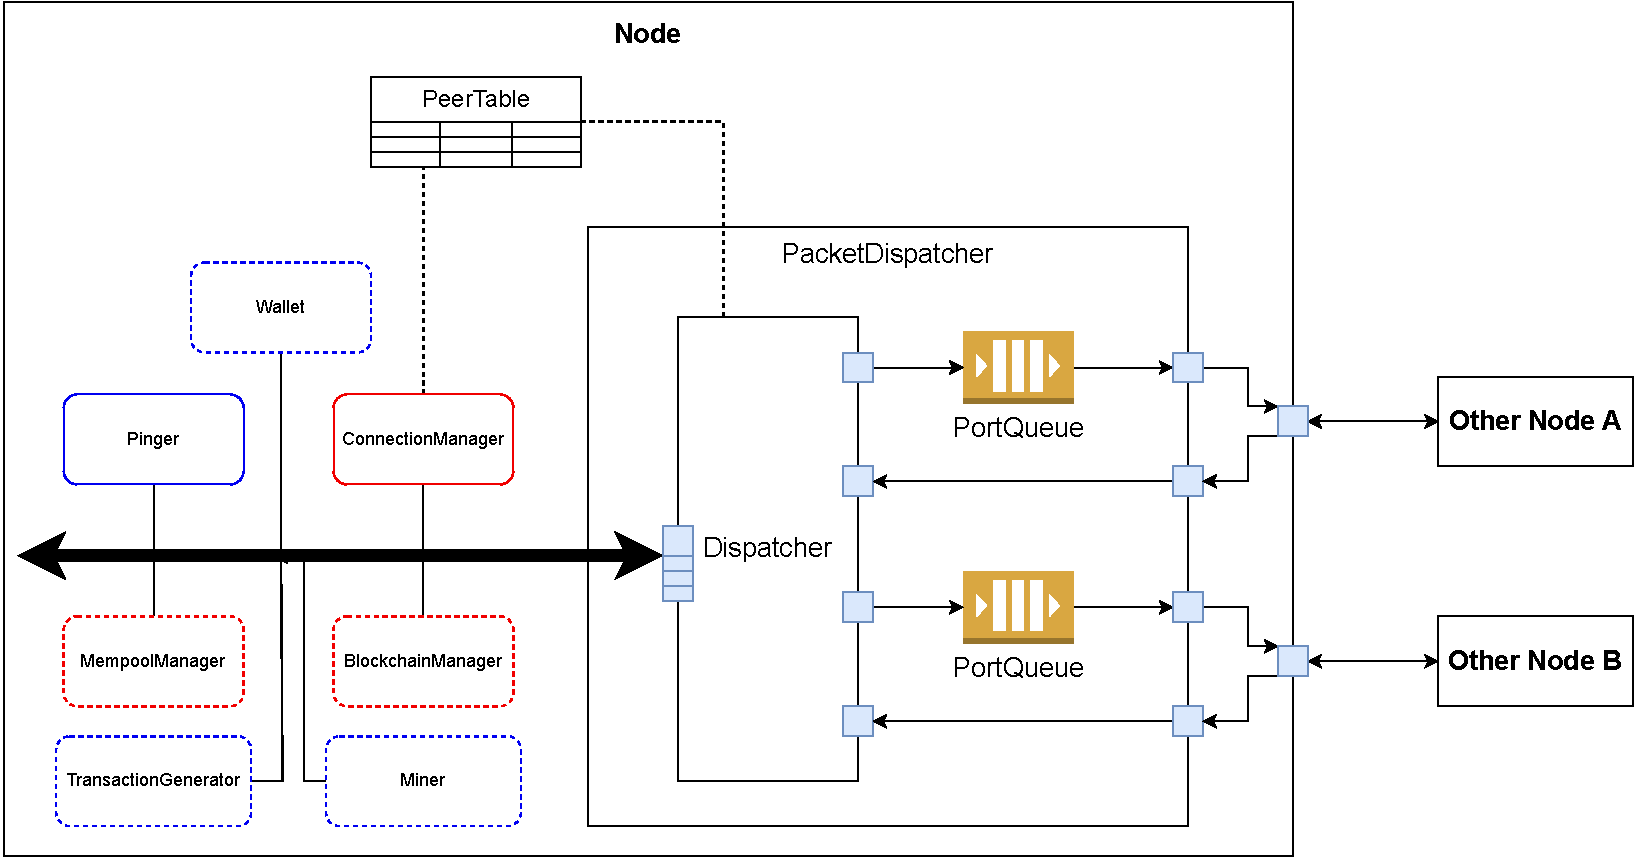
\includegraphics[width=\textwidth]{next-node}
	\caption{The new structure for nodes, supporting \omnetpp{} links.
	Applications now receive and send messages through the
	\code{PacketDispatcher}. Applications with dashed border actually does
	not support this setup in \iblock{}: only the \code{Pinger} and
	\code{ConnectionManager} modules are working.}\label{fig:next-node}
\end{figure}

The \code{Dispatcher} module is responsible for sending outgoing messages to
peers and forwarding incoming messages to applications. Messages exchanged
between nodes are instances of the \code{Packet} class, which encapsulate a
\emph{payload} (instance of the \code{payloads::Payload} class). When the
\code{Dispatcher} receives a \code{Packet}, encapsulates it in another type of
message, the \code{IncomingMessage}, and forwards it to the applications
interested in that type of message.

Applications, during network initialization, call the \code{registerListener()}
method of the \code{Dispatcher}, passing the type of messages they are
interested in. The \code{Dispatcher} then keeps a list of listeners and, when a
message arrives, forwards it to all listeners that are interested in that type.

The \code{AppBase} class already implements different methods to handle
different type of payloads. For example, an application that wants to handle
the \code{Version} message must implement the \code{handleVersionPacket()}
method that will be automatically called when a \code{Version} message
arrives. This also explains the name \code{handleOtherMessage()} used in
\secref{subsec:applications}, as ``other'' means that it is not a protocol
message recognized by the \code{AppBase} class (it is, in fact, a direct
message containing a block or a transaction).

The \code{AppBase} class also supports some methods used to easily send new
messages to peers. Packets to be sent to other peers are encapsulated in
\code{OutgoingMessage} messages and the forwarded to the \code{Dispatcher}. The
\code{OutgoingMessage} class contains the packet to transmit and information
on the destination peer (or peers) taken from the peer table.

The dispatcher is actually a compound module (\code{PacketDispatcher}) that
contains the \code{Dispatcher} module and one or more \code{PortQueue} modules.
The \code{PortQueue} module is used to store messages that are waiting to be
sent to peers. Each gate has a corresponding \code{PortQueue} module which is
needed since, during transmission, the links are \emph{busy} and cannot
transmit another message at the same time. So messages are queued and sent one
at a time.

\subsection{Protocol Handshaking}\label{subsec:handshaking}

The peer table needs to be filled with informations about the peers. This work
is done by the \code{ConnectionManager} module, which is responsible for the
initial handshake with other nodes. The \code{ConnectionManager} module
implements the same protocol handshaking mechanism as in the real Bitcoin
protocol, which is quite simple: when a node connects to another node, it sends
a \code{Version} message containing informations about itself. The other node
replies with a \code{Version} message, containing its own informations, and a
subsequent \code{Verack} message to acknowledge the reception of the first
message. Finally, the first node sends a \code{Verack} message to acknowledge
the reception of the second \code{Version} message.

This mechanism is implemented in the \code{ConnectionManager} module by
overriding the \code{handleVersionPacket()} and \code{handleVerackPacket()}
methods of the \code{AppBase} class. The handshake with another node is started
when the \code{connect()} method of the \code{ConnectionManager} class is
called by the \code{AppBase} class. The method is called automatically when the
user's code in the application wants to send a message to a peer and the peer
has not been connected yet. This way the handshaking process is totally
transparent to the application.

The message that the application wants to send to the peer is kept in a queue
by the \code{AppBase} until the handshaking is completed. When the handshaking
completes, the message is sent to the peer, always encapsulated in a
\code{OutgoingMessage} sent to the \code{Dispatcher} that decapsulates it and
sends out the \code{Packet} to the gate connected to the peer, as stored in the
peer table.

\subsection{Ping-Pong Example}\label{subsec:ping-pong}

The \code{Pinger} module support the exchange of \code{Ping} and \code{Pong}
messages of the Bitcoin protocol specification. The application sends
periodically, with a configurable interval, a \code{Ping} message to a random
peer taken from the peer table and waits for the \code{Pong} reply, which is
done by the \code{Pinger} module of the other node.

If the node is not connected to the peer \idest{the node and the peer still
needs to do the initial handshaking}, \code{AppBase} will queue the \code{Ping}
message and ask the \code{ConnectionManager} via a DMC to start the handshaking
process. The \code{Ping} message will be sent to the peer as soon as the
handshaking completes.

\figref{fig:ping-pong} shows an example network with 6 nodes connected via
\omnetpp{} links and exchanging ping-pong messages.

\begin{figure}[tbhp]
	\centering
	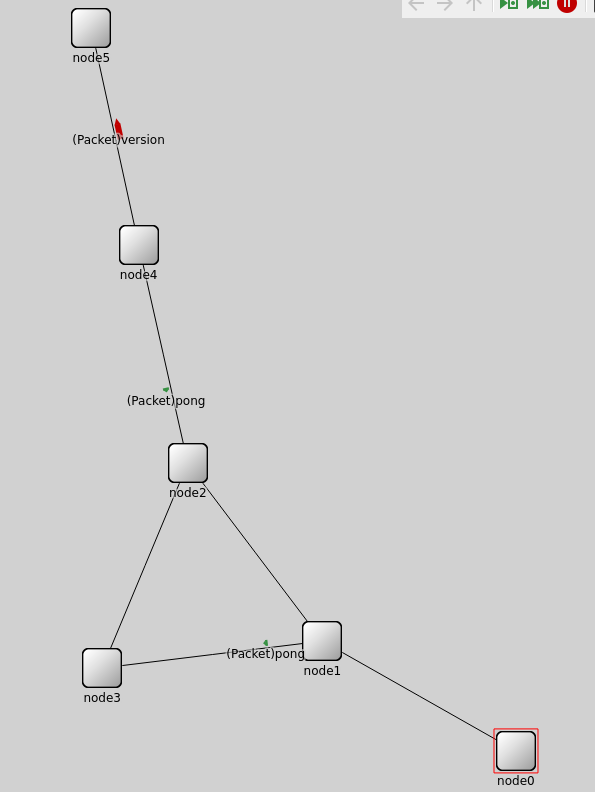
\includegraphics[width=\textwidth]{ping-pong}
	\caption{Example network with 6 nodes exchanging ping-pong
	messages. We can also see a node exchanging a \code{Version} packet
	with one of its peers.}\label{fig:ping-pong}
\end{figure}
